\part{Aspectos Gerais}
\chapter[Introdução]{Introdução}
Controle, uma palavra chave para que um bom projeto seja desenvolvido. Um projeto consiste em um processo único que tem como objetivo um produto inovador de um grupo de afazeres sincronizados e gerenciados em um determinado período de tempo. A disciplina Projeto integrador 1 busca por meio dessas características mostrar como deve ser a realização do projeto.

Mediante os atributos a turma A irá elaborar o projeto de um Prédio sustentável e inteligente com o objetivo de trazer conforto para todos os que utilizarem da Faculdade do Gama, o projeto consiste em sanar problemas já enfrentados pelo corpo discente e docente da universidade como por exemplo iluminação má planejada, sistema de chamada em papel o que causa uma grande perca de tempo por parte do professor, desperdícios energéticos e hídricos no campus também serão solucionados no projeto.

O Prédio sustentável inteligente consiste em utilizar fontes de  energia e materiais sustentáveis,visto que atualmente a sustentabilidade é um ponto crucial para um bom desenvolvimento da sociedade. Por meio de softwares e sistemas eletrônicos pretende-se monitorar desperdícios hídricos e energéticos construindo assim uma sistema Smart Grid na universidade além de criar um sistema de controle e acesso que evite fraude e que o professor não perca tempo para executá-lo.

Dessa forma, com as engenharias do campus trabalhando de forma harmônica tem-se como objetivo melhorar o ambiente de trabalho e de estudos para os que frequentam o campus da FGA , fazendo assim que os professores e os alunos tenham ferramentas e ambientes favoráveis para realizar uma boa didática e boas pesquisas.

\section{Descrição do Problema}
A Universidade de Brasília, é umas das faculdade mais importantes do Brasil, desfrutando de vários campi em diversas regiões administrativas do Distrito federal. A Faculdade do Gama, um dos campi da UnB, é considerada o campus da tecnologia pois hospeda as engenharias mais modernas: Engenharia Automotiva, Aeroespacial, Eletrônica, de Energia e de Software. Lamentavelmente o campus enfrenta problemas que dificultam o desenvolvimento de tecnologia.

Apesar de ter um ótimo corpo docente, o campus da FGA possui algumas deficiências no que diz respeito à estrutura e tecnologia. Ainda que seja relativamente jovem, já podem ser observadas rachaduras na estrutura de todos os pŕedios. Além disso, o dimensionamento das salas e posicionamento de lousas, projetores e a má iluminação também são problemas enfrentados no cotidiano dos que utilizam a salas e laboratórios.

Ademais, a Faculdade do Gama enfrenta problemas de superlotação. No primeiro semestre de cada ano, ingressam cerca de 280 alunos (140 por meio do SiSU \cite{sisu} e 140 por meio do PAS \cite{pas}). Ainda que haja uma taxa de evasão de aproximadamente 15 \% \cite{evasao} no campus, a atual estrutura é incapaz de acomodar toda demanda.

Ironicamente, a falta de tecnologia é outro problema enfrentado. A falta de equipamentos necessários para realização de aulas e da atividade de pesquisa. Além disso, o processo de chamada é feito de um modo arcaico e passível de erros e fraudes, o que exige tempo e esforços dos professores.

Por fim, outra adversidade observada é o controle de acesso à faculdade. Tendo em vista que que qualquer pessoa pode acessá-la sem nenhum monitoramento, o ambiente é comumente assaltado e vandalizado.

\chapter{Requisitos\label{ch:requisitos}}

A Engenharia de requisitos estuda como coletar, entender, armazenar, verificar e gerenciar requisitos. Sua principal preocupação é entender e documentar quais são os requisitos reais do sistema \cite{belgamo2000}. Ela é dividida em diferentes fases: Elicitação, Análise, Especificação, Verificação e Gerenciamento.

A Elicitação é definida como o processo de  compreensão dos requisitos dos steakholders \cite{yousuf2015}, e é o primeiro estágio para a construção do entendimento sobre o problema. Para isso existem diferentes técnicas para que os requisitos sejam coletados de maneira correta e eficiente. Neste projeto foram utilizadas duas técnicas:
Questionário e Brainstorming.

A aplicação de questionários é um dos métodos de elicitação de requisitos de menor custo. Esta técnica costuma alcançar uma grande quantidade de pessoas, em menos  tempo e com baixo custo \cite{gunda2008}. Para aplicar esta técnica foi utilizada a ferramenta Google Forms, que permite o compartilhamento do questionário em diversas redes sociais. As respostas são fornecidas pela plataforma em texto, quando as questões são dissertativas, ou em gráficos, como mostra a figura a seguir.

\begin{figure}[h]
  \caption{Questionário sobre problemas da FGA}
  \centering
    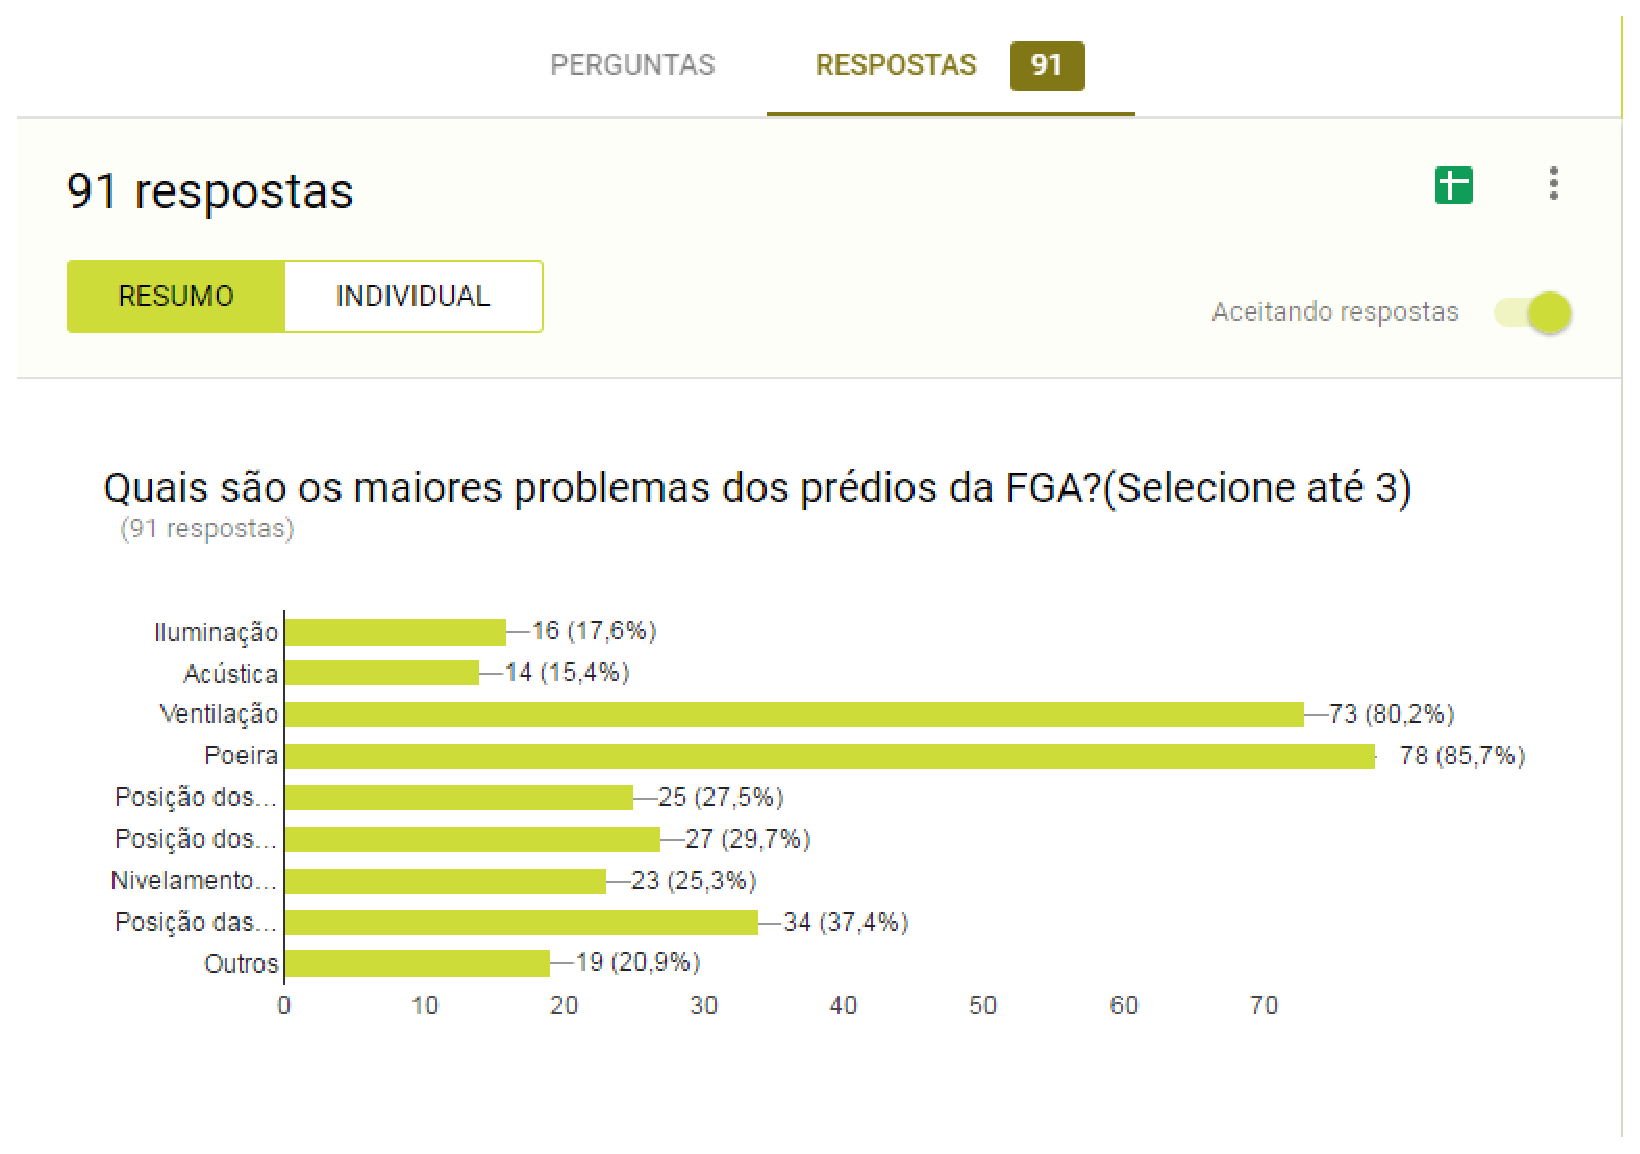
\includegraphics[width=1.0\textwidth]{figuras/pesq.eps}
\end{figure}

Brainstorming é uma técnica de grupo utilizada para criar novas ideias para o projeto e/ou encontrar soluções para um problema específico, além de possibilitar o diagnóstico de problemas em pouco tempo. São conduzidos como uma conferência reunindo de seis a dez membros, onde cada membro tem o direito de explanar suas ideias em um certo período de tempo. Esta reunião possui um mediador, que define a questão a ser discutida \cite{gunda2008}.

Esta técnica foi aplicada por meio de uma reunião com toda a equipe, onde, baseadas nos requisitos fornecidos na descrição do projeto do prédio inteligente, as ideias geradas foram anotadas em um documento editável no Google Drive. Ao longo da semana, todos os membros da equipe poderiam continuar escrevendo suas ideias no documento, que foram discutidas e priorizadas na aula seguinte, novamente com toda a equipe. Nesta reunião foi realizada a Análise dos requisitos gerados pelas técnicas de elicitação.

Estes requisitos foram documentados no Backlog do Produto, mostrado na figura ~\ref{fig:backlog}, onde os requisitos foram agrupados visando a rastreabilidade vertical, partindo de grandes blocos mais genéricos chamados Épicos, que são divididos em partes menores chamadas Features.


\chapter{Escopo}
Para a realização do projeto Prédio inteligente deve-se definir as especificações do limite que contempla o projeto, para isso foi necessário definir os requisitos e analisá-los e aplicar alguns métodos para facilitar a definição do escopo como o dos 5W e 2H representado abaixo:

1-What -O que será feito ?

2-Who- Por quem será feito ?

3-Where- Onde será feito ?

4-When-Quando será feito?

5-Why-Por que será feito?

6-How-Como será feito ?

7-How Much- Quanto custará?

    Dessa forma o escopo foi definido como sendo o Prédio Sustentável inteligente da Faculdade do Gama(FGA) e pode ser melhor observado na EAP visto que a mesma guia a equipe para o término do projeto,não incluindo geração de energia ou algum sistema tecnológico para outra parte do campus exceto o estacionamento parte fundamental do campus que ainda não foi concluída e pode ser resolvida com ideias que possuem nesse projeto , esse escopo foi decidido com base: no  alto custo financeiro para suprir toda demanda energética do campus, futuras alterações de estruturas e dimensões dos prédios já construídos e pelo tempo de entrega do projeto.Por fim,foi realizado um escopo para que futuramente a Universidade de Brasília pudesse aproveitá-lo para a construção do novo prédio trazendo assim conforto e ferramentas necessárias para todos que necessitam do mesmo para absorver conhecimento.(stakeholders).
    Outra subdivisão do nosso projeto, trata da parte de controle de acesso, que é responsável por monitorar todo o acesso de pessoas feito neste nosso prédio tecnológico dentro da FGA. Levando em conta que o nosso trabalho é feito em uma universidade federal, não podemos fechar completamente o acesso à universidade, entretanto nosso objetivo é selecionar quem terá ou não acesso a partes específicas dentro do novo prédio.

Inicialmente a ideia é restringir uma parte do estacionamento só para alunos matriculados na faculdade, e para que seja liberada a entrada, é necessário a liberação automática mediante apresentação de carteirinha, em seguida, o acesso também será restringido nas salas e laboratórios com trancas que serão acopladas nas portas, no caso de laboratórios e salas com equipamentos mais sofisticados, somente será autorizada a entrada com um professor como responsável pelo uso do ambiente, e no caso das salas simples, também haverá necessidade de um responsável, contudo, poderá ser tanto aluno, monitor ou professor. A frequência também será averiguada mediante carteirinha em um aparelho eletrônico portátil que cada professor possuirá. Essa tecnologia e modo de segurança já é utilizado em várias universidades do mundo e especialmente em algumas faculdades particulares em Brasília e por isso é uma ideia a ser implementada dentro da UnB principalmente por questão de segurança.

Na parte estrutural do projeto serão aplicados materiais inteligentes e sustentáveis para amenizar a produção de resíduos e consequentemente o impacto no meio ambiente. Além disso, serão consideradas algumas adaptações sobre o uso das salas para se possa receber o sistema de automação e também quais serão destinadas a laboratórios ou salas de aula, de acordo com as necessidades dos usuários. Por fim, haverá a alteração da posição dos elementos usados em sala para melhorar o impacto que os mesmos têm no aprendizado.

Para a produção energética foi considerada duas formas para suprir a demanda energética da FGA a primeira e principal é a geração de energia por meio de placas fotovoltaicas e a segunda sendo utilizada como reserva será por meio de um gerador movido a biodiesel.

\section{Backlog do Produto}
Conforme discutido no capítulo \ref{ch:requisitos}, o \textit{backlog} do produto foi definido com os requisitos agrupados em uma rastreabilidade vertical, seguindo do mais abstrato (ou alto nível) para o mais específico (ou baixo nível).

\begin{figure}[!h]
  \centering
  	\includegraphics[width=0.9\textwidth]{figuras/backlog.eps}
   \caption{Backlog do Produto\label{fig:backlog}}

\end{figure}

\chapter{Metodologia}
\section{Introdução}
\begin{quote}
\textit{“Ninguém, com toda certeza, é capaz de assumir a liderança em todos os campos, pois para um homem os deuses concederam as proezas da guerra, a outro, a dança, para um outro, a música e o canto, e, num outro, o todo poderoso Zeus colocou uma boa cabeça”} - Homero
\end{quote}

\vspace{\onelineskip}
\vspace{\onelineskip}

A administração de pessoal foi caracterizada como uma das atividades mais exigentes deste projeto, devido ao tamanho da equipe: 35 alunos. Portanto, organização do time tornou-se crucial para o bom desenvolvimento do projeto.

Ademais, nenhum membro participante jamais trabalhou em um projeto desta dimensão, portanto não há experiência prévia quanto à administração e liderança.

Esses foram motivos que levaram à escolha de uma gestão descentralizada. A metodologia aqui escolhia foi baseada no SAFe, framework que será descrito posteriormente.

Designou-se cinco líderes para os grupos formados (descritos em \ref{subsec:divisao}). Todas as decisões são tomada, então, à partir de um conselho de líderes (ou gerentes), ao invés de apenas um membro. Foi designado, ainda, um gerente geral (externo aos grupos e, portanto, imparcial), para a tomada de decisões em caso de eventualidades. Se, porventura, houver alguma discordância entre os membros da gerência, será realizado uma reunião destes com o gerente geral, que auxiliará na tomada de decisão mais adequada.

\section{Scaled Agile Framework (SAFe)}
SAFe é um framework que propõe boas práticas de desenvolvimento ágil, tendo uma estrutura baseada em práticas e padrões
 propostos e consolidados em outros frameworks, como: Lean, XP (eXtreme Programming), Scrum e Kanban \cite{dasilva2016}.

Este framework suporta o desenvolvimento em pequenas escalas (menos de 100 pessoas), mas tem o grande foco no desenvolvimento
empresarial com grandes e complexas produções de software.

Derivados dos lean e ágil, o SAFe apresenta os seguintes princípios:
\begin{itemize}
 	\item Adotar uma visão econômica
 	\item Aplicar pensamento sistêmico
 	\item Assumir variabilidade
 	\item Construir gradualmente com ciclos de aprendizagem rápidos e integrados
	\item Marcos básicos na avaliação objetiva dos sistemas de trabalho
	\item Visualizar e limitar WIP, reduzir tamanhos de lote e gerenciar comprimentos de fila
	\item Aplicar cadência, sincronizando com o planejamento entre domínios
 	\item Desbloquear a motivação intrínseca dos trabalhadores do conhecimento
 	\item Descentralizar a tomada de decisão
\end{itemize}

 O SAFe apresenta diversos benefícios, como aceleração do time-to-market, aumento da produtividade e da qualidade, e
 redução de riscos e custos do projeto \cite{turetken2016}.

 \begin{figure}[!h]
 	\centering
 	\includegraphics[keepaspectratio=true,scale=0.17]{figuras/safe.eps}
 	\caption{SAFe}
 	\label{fig01}
 \end{figure}

\section{Integração Entre as Engenharias}
Por ser um projeto feito no tronco comum de matérias da universidade, este dispõe de habilidades e conhecimentos de todas as engenharias disponíveis: software, energia, eletrônica, aeroespacial e automotiva.

Somado à isso, o fato do projeto tratar-se de um prédio sustentável e tecnológico permite a participação de todas as engenharias trabalhando juntas, visto os muitos aspectos que tal edificação demanda.

Em primeiro plano, a Engenharia de Energia trabalha principalmente com a solução Smart Grid do projeto, fazendo com que toda a solução energética seja inteligente e trabalhe com a possibilidade de falhas. A Engenharia Eletrônica trabalha na parte de instrumentação eletrônica, como mesas inteligentes, sensores de presença nas salas, e no controle de acesso ao prédio. Em relação às Engenharias Aeroespacial e Automotiva, existe pouca aplicação direta do seu conhecimento no projeto. Todavia, há muita contribuição indireta desses grupos principalmente na área de estrutural do ambiente, isto é, na formação física da construção, a forma em que serão organizadas as salas e laboratórios, os materiais mais adequados ao uso, entre outros fins. Por outro lado, a Engenharia de Software trabalha como um elo de todo o projeto, uma vez que todas as áreas dependem, direta ou indiretamente, de um sistema que processe as informações e as disponibilizem para os interessados.

Em síntese, a interação das engenharias no projeto é claramente vista, em consequência da diversa gama de conhecimento necessária para a idealização, projeção e construção do prédio. É importante ressaltar que, ainda que uma área não trabalhe diretamente com uma das engenharias, sua contribuição será indireta em outros âmbitos.

\subsection{Divisão de Grupos\label{subsec:divisao}}

Com base na interdisciplinaridade de todas as áreas, a turma optou por não dividir grupos com base nos cursos, e sim em áreas de conhecimento e atuação. Dessa forma, duas ou mais engenharias puderam se agrupar de modo a maximizar a diversidade de conhecimentos envolvidos, propondo uma solução mais adequada ao projeto.

A divisão dos grupos ficou como se segue:

	\begin{itemize}
		\item \textbf{Estrutura e Materiais:} Responsável pela escolha e aplicação de materiais inteligentes na estrutura, otimização da planta e organização do espaço interno.
		\item \textbf{Smart Grid:} Responsável pela a  escolha e dimensionamento, de forma eficiente, do tipo de energia a ser utilizada para suprir a demanda energética da FGA.
        \item \textbf{Automação 1 - Controle de Acesso:} Responsável pelo controle de acesso à universidade, salas e laboratórios, além do registro de frequência durante as aulas.
        \item \textbf{Automação 2 - Instrumentação e Controle:} 	Responsável pela implantação dos dispositivos de instrumentação e controle do prédio. Isto engloba sensores, equipamentos de automação das salas e os equipamentos de controle e processamento destes dados.
        \item \textbf{Interfaces e Processamento de Software:} Responsável pelo processamento de todos os dados fornecidos pelos grupos anteriores, bem como sua disponibilização aos usuários por meio de interfaces gráficas.
	\end{itemize}


\chapter{Ferramentas}
Comunicação é parte essencial de um projeto, especialmente em um baseado em metodologias ágeis. Segundo Potsch \cite{potsch2009}, de 2005 a
 2008 a comunicação foi reiteradamente considerada como o problema mais freqüente no gerenciamento de projetos.

Em vista disso, a comunicação entre os membros do projeto foi explorada em todos os mecanismos disponíveis, sejam eles físicos ou virtuais.
	Segue-se uma breve descrição das ferramentas utilizadas para a gestão do projeto e das equipes participantes, bem como o propósito delas.

\section{Comunicação}
Ferramentas de comunicação utilizadas:

	\begin{itemize}
		\item \textbf{Google Hangouts:} Ferramenta de comunicação em chat e videoconferência. Utilizada para reuniões não presenciais entre as equipes.
		\item \textbf{Whatsapp:} Aplicativo de troca de mensagens instantâneas para celular. Utilizado para comunicação rápida e/ou informal entre as equipes do projeto.
	\end{itemize}

\section{Rastreabilidade}
Ferramentas de rastreabilidade utilizadas:

	\begin{itemize}
		\item \textbf{Google Drive:} Ferramenta de armazenamento e compartilhamento de documentos, apresentações, formulários entres outros tipos de arquivo. A ferramenta utilizada para o compartilhamento e confecção de documentos.
		\item \textbf{Podio:} Plataforma usada para administração de empresas, projetos, recursos humanos, finanças entre outros fins. Nesta plataforma disponibiliza vários aplicativos que tem funções de acordo com a necessidade do usuário. Para o projeto serão usados os aplicativos Kanban, Calendário e a função de Tarefas. O primeiro aplicativo será utilizado para gerenciar as tarefas a serem realizadas. O segundo será usado para controle do cronograma e datas de entrega, e o último aplicativo para delegação de tarefas. É possível que mais algum aplicativo venha a ser utilizado de acordo com as necessidades da equipe.

	\end{itemize}

\chapter{EAP}
	A Estrutura Analítica de Projetos (EAP), é uma ferramenta visual que é feita a partir da decomposição das etapas do projeto em ordem cronológica. Ela funciona como um facilitador para a identificação de cada etapa do projeto, facilita os processos de gerenciamento e entregas bem como a estimativa de esforço, custo e duração do mesmo. Além da principal função, a definição do escopo do projeto. A EAP é representada em diagrama, começando do tópico mais geral, em seguida as principais etapas, e por fim as entregas que cada etapa necessita.

Para o projeto do Prédio Inteligente elaborou-se uma EAP para que fosse mais fácil a visualização das etapas que devem ser seguidas, além da definição do escopo do mesmo. Essa ferramenta também serve para que todos da equipe tenham acesso à modo que o projeto será desenvolvido. Sendo assim, as fases principais foram divididas em: Planejamento, Justificativa das Soluções e Viabilidade Econômica. Implicitamente estas fases representam os Pontos de Controle 1, 2 e 3 respectivamente. Consequentemente, foram definidas as entregas que devem ser feitas para cada Ponto de Controle.
 \begin{figure}[!h]
 	\centering
 	\includegraphics[keepaspectratio=true,scale=0.37]{figuras/eap.eps}
 	\caption{EAP do Projeto Prédio Inteligente}
 	\label{fig01}
 \end{figure}

\chapter{Canvas}
O Canvas é uma ferramenta de planejamento estratégico criada para esboçar modelos de negócio. Essa ferramenta é um mapa visual de novo blocos
que descrevem o modelo de negócio que o usuário deseja produzir.

Segue-se o Canvas elaborado para este projeto.

\begin{figure}[!h]
 \centering
 \includegraphics[keepaspectratio=true,scale=0.35]{figuras/canvas.eps}
 \caption{Canvas do Projeto Prédio Inteligente}
 \label{fig031}
\end{figure}
